\subsection{RabbitMQ [VI]}

RabbitMQ is a queue messaging server \cite{RabbitMQ, AlvaroWilliams2012}.
It provides a robust, efficient and scalable message broker that serves as an intermediate layer between sending and receiving clients.
RabbitMQ has a simple data model that, nevertheless, offers flexibility in the structure of data flows.
It gives an opportunity to adjust a tradeoff between throughput and reliability.
RabbitMQ fully applies Advanced Message Queuing Protocol (AMQP).

RabbitMQ is basically a delivery system, that receives messages, handles them, and then sends them to the destinations.
It is called also a \textit{broker server}\mnote{Broker server}.
It can serve messages coming from client apps to a server and backwards.
It also can be a mediator between client apps themselves.
RabbitMQ rules messages going through it, so that they are reliably stored, distributed, and then sent, possibly many times in case of absence of acknowledge from the destination.
It completely separates senders and receivers, so that they can be easily modified, removed, or added.
Figure~\ref{fig:RabbitMQGeneralStructure} shows general structure of RabbitMQ server and the flow of messages.

\begin{figure}[h]
  \centering
  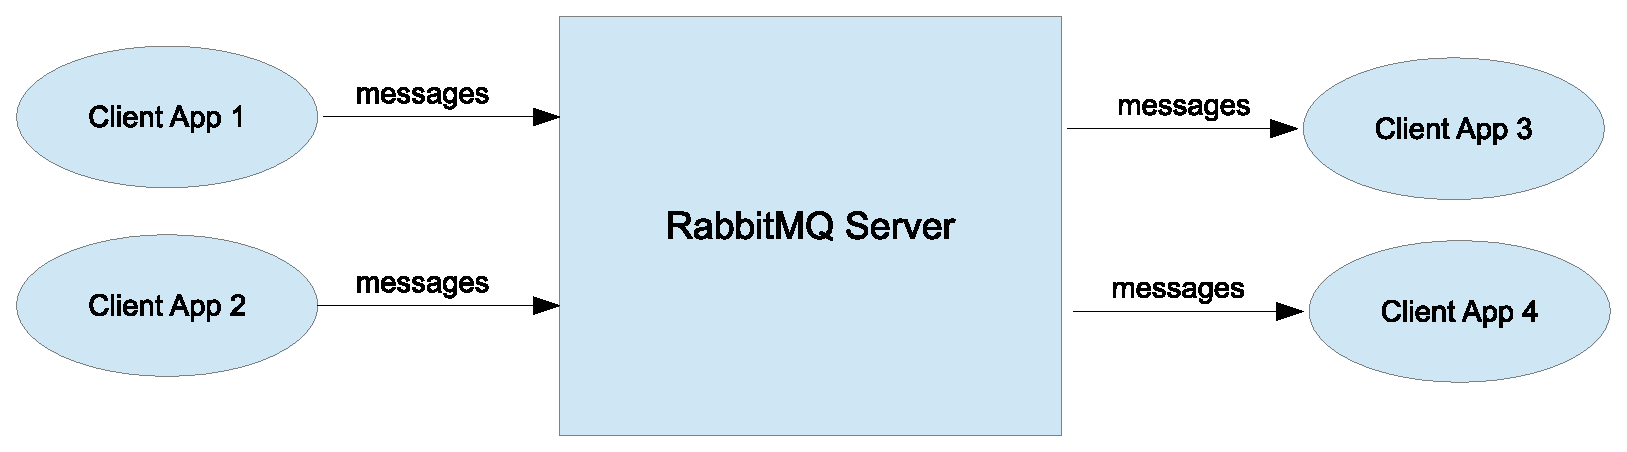
\includegraphics [width=0.9\textwidth]{images/RabbitMQGeneralStructure}
  \caption{General structure of RabbitMQ server and the flow of messages.}
  \label{fig:RabbitMQGeneralStructure}
\end{figure}

Client that sends messages is called \textit{producer}\mnote{Producer}.
Producer creates a message and sends (publishes) it to a broker.
Message consists of two parts: label and data.
Data can be anything, e.g. text, JSON object, JPG file, etc.
Label provides information about who should receive the message.
When producer sends a message, it does not wait for a confirmation from supposed receivers.
Such strategy is called fire-and-forget.
Broker acknowledges only the fact, that it has received the message properly.
It does not provide information to a sender about further life of the message. 

Client that receives messages is called \textit{consumer}\mnote{Consumer}.
Consumer subscribes to a specific \textit{queue} (we discuss queues in details below).
Broker transmits messages, coming to this queue, to all subscribed consumers.
There is no way to know who was a publisher of a message using label.
The only possibility is to sign this message inside of the data part, what is, basically, not in the scope of broker's responsibilities.

The same application can be a producer and a consumer at the same time.
This is often a case, because application usually needs to communicate with the server or with other nodes of the network using broker server.
But it is important to mention, that there are, basically, no client and server notions in the discussed concept.
Rather it is a model of publishers and subscribers, or senders and receivers.
Broker server acts then as a middle transport layer.

For further discussion we need to describe \textit{Advanced Message Queuing Protocol} \mnote{Advanced Message Queuing Protocol (AMQP)} or \textit{AMQP} \cite{AMQP2011}.
AMQP is a protocol that specifies common rules for messaging, queuing, publication/subscription, routing, etc.
It provides reliable, efficient, flexible, generic mechanisms for communication between clients.
AMQP is a binary protocol.
It has a set of commands, that must be implemented, e.g. \lstinline{open}, \lstinline{begin}, \lstinline{attach}, \lstinline{transfer}, \lstinline{flow}, \lstinline{disposition}, \lstinline{detach}, \lstinline{end}, \lstinline{close}.

In order to start publishing messages producer has first to connect to a broker.
It establishes TCP connection, and initializes \textit{AMQP channel} \mnote{AMQP channel} on top of it.
Such channel is only a virtual connection.
Producer can create many AMQP channels in parallel using one TCP connection.
This is useful, when for example one application needs to send many messages to the server from different threads.
It would be then very expensive to establish separate TCP connection for every thread.

Another important element of RabbitMQ broker server is Queue\mnote{Queue}.
It stores messages that are still not delivered.
Also, queue is a named object, and the name is an identifier for consumers, that want to subscribe to this queue.
There are two ways for a consumer to receive a message from the queue.
The first one is to subscribe to a queue and receive all messages that comes in it automatically.
This creates an AMQP channel, that is then used during the whole time of listening.
The second one is to retrieve a single message from a queue.
Consumer acknowledges received message to a broker.
In some cases it can reject message, for example when an error during its processing occurred.
It is then important to specify (rejecting the message), that message must be sent to this consumer once more.

Consumers and producers can create queues.
Consumer must be unsubscribed from any other queue, declaring a new one.
Creating a queue, the one who does it must specify its name (or say to a broker to put random one and return it).
The name is important for producers, that want to publish to this queue.
There are two parameters to mention, that can be also specified.
The queue can be declared as exclusive, what means that only creating consumer is allowed to listen from it.
Another property is auto-deletion, that says to a server, that queue must be deleted after the last consumer unsubscribes from it.

\textit{Exchange} \mnote{Exchange} is a component of RabbitMQ broker server that completes the whole picture.
Exchange is a place to where producer sends a message.
It is then redirected using specific rules to a particular queue.
Those rules are called \textit{routing keys}\mnote{Routing keys}.
It is said, that queue is bounded to an exchange by a routing key.
Each message that producer sends to a broker, has a routing key in its label.
Broker server tries then to match it with its bindings, to put the message in a proper queue.

There are four types of exchanges in RabbitMQ: direct, fanout, topic and header.
The difference between them is in the routing algorithm.
\textit{Direct exchange} simply matches routing key with the queues' names.
Messages go then to the corresponding queue, always to only one among existent.
In the broker server there is always a default direct exchange, but it is possible to create more in case of specific needs of a system.
\textit{Fanout exchange} puts a message to all queues bounded to it.
It is useful, when the message must cause several different reactions.
\textit{Topic exchange} allows to send messages from different sources to the same queue, and to send messages from one source to several queues.
It is the most flexible and powerful type of exchange.
Different interesting messaging scenarios can be realized via topic exchange.
\textit{Header exchange} is similar to direct exchange, but rarely used, and we do not discuss it here.

Important concept in RabbitMQ is \textit{virtual host}\mnote{Virtual host}.
It is, basically, a virtual machine inside RabbitMQ server that serves as a separate broker.
This concept allows to separate different systems having the one RabbitMQ server.
Each virtual host has its completely own set of exchanges, queues and bindings.
It is easy to move virtual host from one RabbitMQ server to another, without necessity to think about what belongs to which broker.

RabbitMQ provides \textit{durability} \mnote{Durability} of broker's structure and existing messages.
If a machine with the RabbitMQ server goes down, or broker just crashes - all exchanges, queues and messages inside will be recovered after restart.
But this mechanism is off by default, and must be switched on, in case durability is important.
To achieve this for every exchange and queue should be set to true parameter \lstinline{durable}.
Also, every message must have a \textit{delivery mode} set to 2, what informs the broker, that it must be persisted in case of crash.
Broker writes then all needed for recovering information to a persistency log file.
It is important to remember, that durability and persistency affect efficiency, that is why they are switched off by default.